\begin{itemize}
    \item
        U und I bei verschiene Lasten, siehe Pflichtenheft.
            ==> Kurven plotten (gemessen und berechnet).
    \item
        Transienten, Laständerungen
    \item
        Leistungsaufnahme
    \item
        Dings funktioniert nicht
    \item
        Structure:
            1) Definition of test fixture
            2) What we actually did
            3) Error analysis
\end{itemize}


There are a variety of tests that can be conducted to verify the performance and
correctness of our  device.  The  following is a list of test fixtures and their
expected results based on simulations.

\subsection{Ripple Voltage and Ripple Current vs Resistive Load}

\begin{figure}[th!]
    \centering
    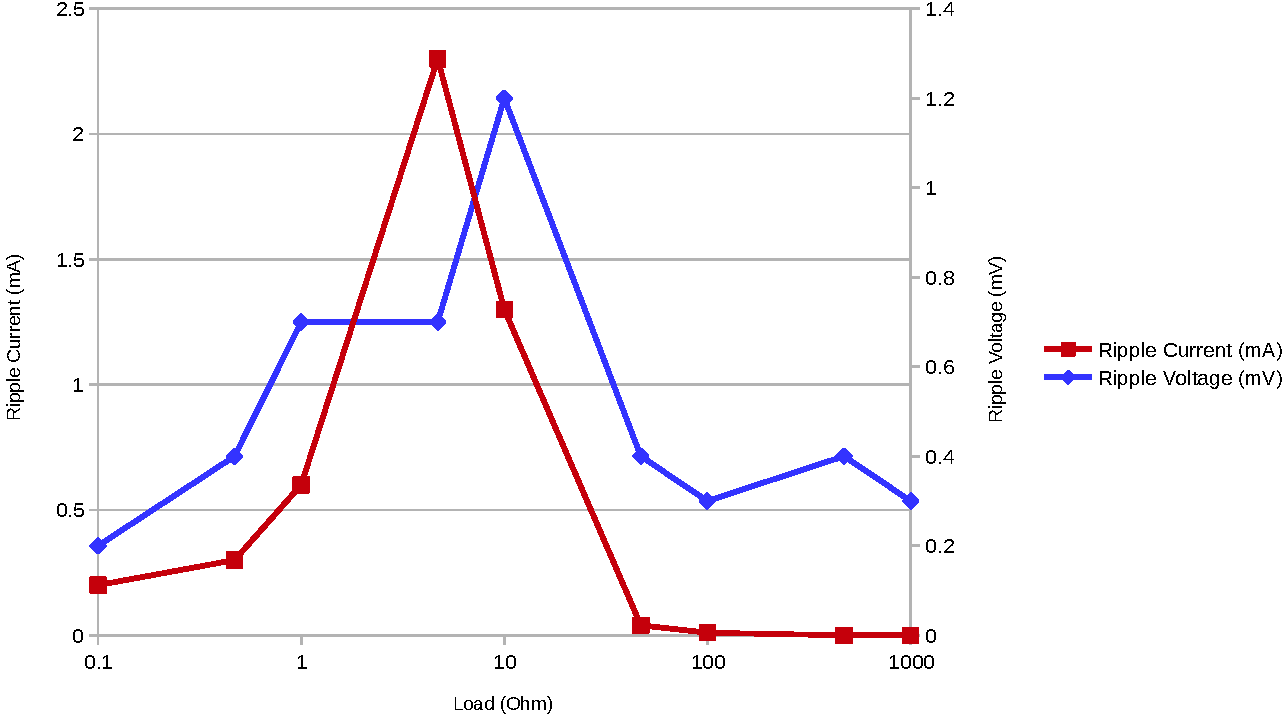
\includegraphics[width=.7\textwidth]{images/sim/ripple-vs-load.pdf}
    \caption{}
\end{figure}

